\documentclass[12pt]{article}

\usepackage{a4wide}
\usepackage[utf8]{inputenc}

\usepackage{graphicx}

%\pagestyle{empty}

\parindent=0pt

\begin{document}

\section*{Filtering Using the Discrete Fourier Transform}

Today's exercise is focused on implementation of simple filters using results of the Discrete Fourier Transform (DFT).

Often the input image is a noise load. This occurs in high frequencies in the frequency domain.
One of the goals of the exercise is to create a filter that removes noise from the input image.
Another task is removing regular vertical bars in the image.

\subsection*{Noise Removal}

As mentioned above, noise is represented by high frequencies of the frequency domain.
From the previous exercise, we have already created an image transform to a frequency domain (DFT) and a reverse conversion to a spatial domain (IDFT).
We now introduce filters into this pipeline.
In the frequency domain, we can apply the following types of filters: low pass, high pass and band pass.
Use low pass filter to remove noise.
Recall that after DFT low frequencies are in corners of the complex matrix and the high frequencies in the center.
In order to our filter to work well, we need to swap 1st with the 3rd quadrant and 2nd with the 4th quadrant (schematically depicted in Fig. \ref{fig:quadrants}).

\begin{figure}[h]
\centering
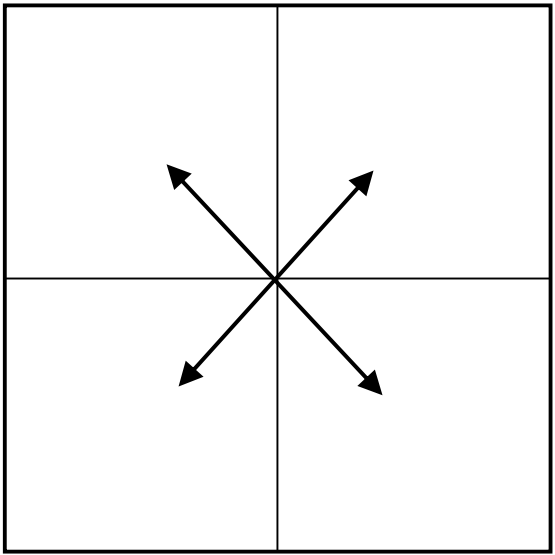
\includegraphics[width=0.25\textwidth]{images/quadrants.png}
\caption{Quadrants swap.}
\label{fig:quadrants}
\end{figure}

Then, you create a mask that has the white color in the circle and the black outside (Fig.~\ref{fig:mask}).

\begin{figure}[h]
\centering
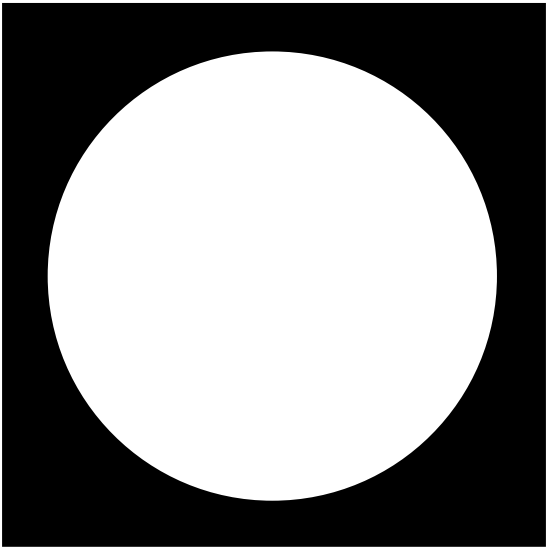
\includegraphics[width=0.25\textwidth]{images/mask.png}
\caption{High pass mask.}
\label{fig:mask}
\end{figure}

The diameter of the circle will depend on filtration rate (try to elabotate on this).
To remove high frequencies (low pass filter), go through the mask's pixels and set the complex matrix to the value of 0 outside the white circle.
Do the reverse for the high pass filter.
After setting the values, you must swap the quadrants back to the original positions.
Result of the low pass filter is shown in Fig. \ref{fig:low_high}.

\begin{figure}[h]
\centering
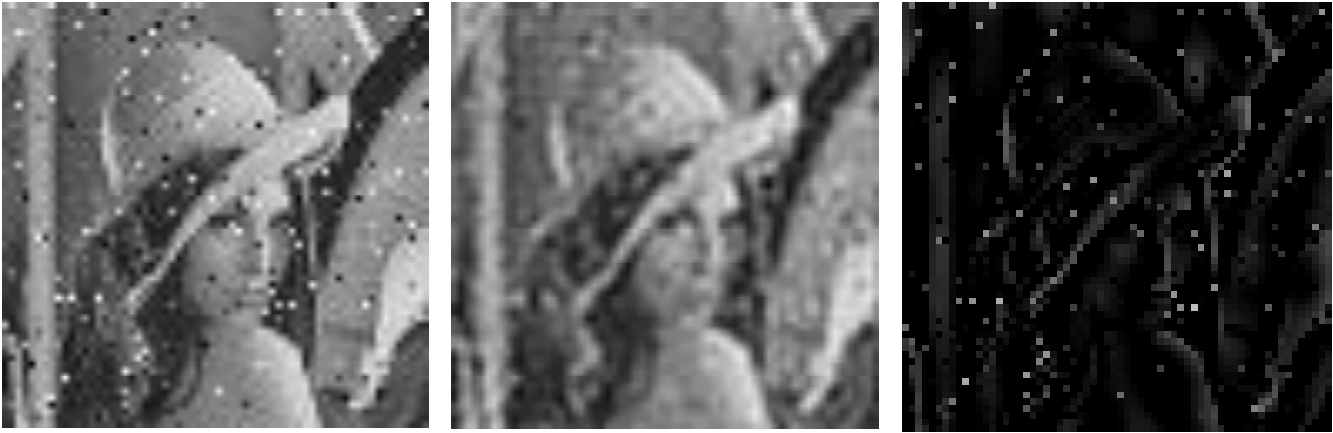
\includegraphics[width=0.8\textwidth]{images/lena_low_high.png}
\caption{Input image (\textit{left}); filtered with low pass (\textit{middle}); filtered with high pass (\textit{right}).}
\label{fig:low_high}
\end{figure}


\subsection*{Removing regular vertical lines}

Now, the situation is somewhat more complex.
Try to figure out the frequencies of those vertical lines in the input image.
Images of the frequecy spectra placed at the exercise's website may guide you to complete this task.
Setting the right parts the complex matrix to 0 can achieve the effect shown in Fig. \ref{fig:lena_bars_example}.

\begin{figure}[h]
\centering
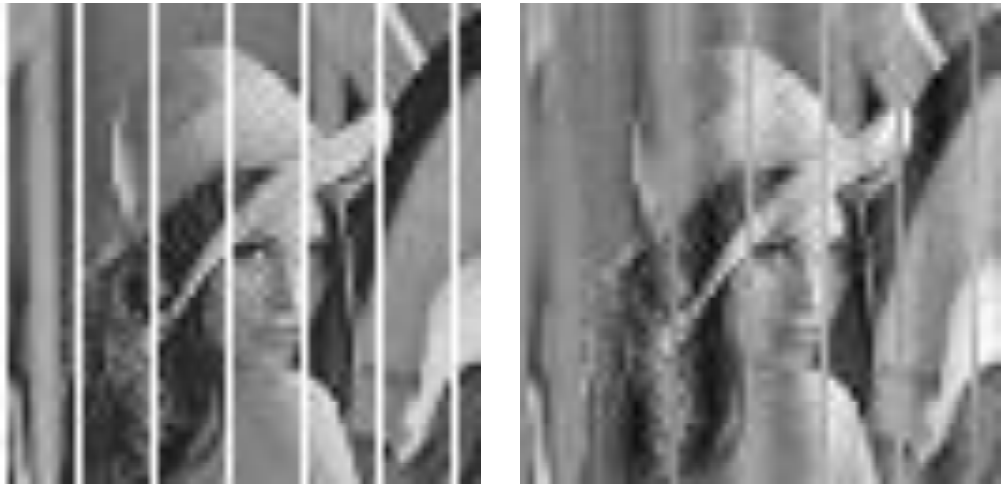
\includegraphics[width=0.6\textwidth]{images/lena_bars_example.png}
\caption{Input image (\textit{left}); removal of vertical bars (\textit{right}).}
\label{fig:lena_bars_example}
\end{figure}

%\section*{Expected Output}

%\begin{center}
%\includegraphics[width=0.8\textwidth]{resultat.png}
%\end{center}

\end{document}

